\documentclass[a4paper,11pt]{article}
\usepackage[utf8]{inputenc}
\usepackage{amsmath}
\usepackage{amssymb}
\usepackage{geometry}
\usepackage{graphicx}
\usepackage{float}
\usepackage{fancyhdr}

\geometry{a4paper, margin=1in}

\title{Conception de base de donnée: Étude de Cas d'une Bibliothèque}
\author{SANNA Thomas, L3STI}
\date{\today}

% Configuration des en-têtes et pieds de page
\pagestyle{fancy}
\fancyhf{}
\fancyhead[L]{Étude de Cas : Bibliothèque}
\fancyhead[R]{\today}
\fancyfoot[C]{\thepage}
\fancyfoot[L]{SANNA Thomas, L3STI}
\fancyfoot[R]{Université de Corse Pasquale Paoli}

\begin{document}

\maketitle

\section{Introduction}
Une bibliothèque municipale souhaite informatiser sa gestion. Suite à divers entretiens et au recueil d'informations sur différents documents utilisés actuellement par la bibliothèque, on a pu élaborer un certain nombre de règles et une liste d'informations qui vont permettre de construire votre MCD (Modèle Conceptuel de Données).

\section{Règles et Informations}
\subsection{Types d'objets}
La bibliothèque gère trois types d’objets : ouvrage, exemplaire et livre. Ces termes sont définis comme suit :
\begin{itemize}
    \item Un \textbf{livre} correspond au titre d'un ouvrage (ex : L’Enfant des lumières, Les Misérables).
    \item Un \textbf{ouvrage} est un terme générique, incluant plusieurs éditions d’un même livre.
    \item Un \textbf{exemplaire} est un livre concret référencé dans la bibliothèque, possédant un numéro d'identification unique. Deux exemplaires d'un même ouvrage peuvent avoir des éditeurs différents, ou appartenir à des collections différentes.
    \item Un livre est identifié par son ISBN.
\end{itemize}

\subsection{Relations et Contraintes}
\begin{itemize}
    \item Un ouvrage peut être écrit par plusieurs auteurs. Pour certains ouvrages, on ne connaît pas l'auteur (cas de la Bible) ; dans d'autres, l’auteur est inconnu.
    \item Un livre peut exister dans plusieurs exemplaires dans la bibliothèque.
    \item Un abonné peut réserver plusieurs ouvrages, mais doit préciser l'ouvrage désiré lors de la réservation. Pour réserver un livre spécifique, il doit indiquer le numéro ISBN du livre.
    \item Un exemplaire peut être emprunté par un abonné, qui doit indiquer la date de retour.
    \item Un emprunt est identifié par le numéro d'abonné et le code de l'exemplaire. La date de retour est mémorisée.
    \item Le directeur connaît les ISBN des livres à commander, et peut passer des commandes avec un fournisseur. Une commande est faite auprès d’un seul fournisseur et contient une quantité de livres.
\end{itemize}

\subsection{Liste d'Informations}
\begin{itemize}
    \item TITRE : titre de l'ouvrage
    \item CODE EXEMPLAIRE : code de l'exemplaire
    \item DATE DE SUPPRESSION DE L’EXEMPLAIRE
    \item NOM EDITEUR : éditeur du livre
    \item ADRESSE EDITEUR
    \item NOM AUTEUR : nom de l'auteur de l'ouvrage
    \item CODE OUVRAGE
    \item PRENOM AUTEUR : prénom de l'auteur de l'ouvrage
    \item DATE DE PRET DE L’EXEMPLAIRE
    \item DATE DE RETOUR DE L’EXEMPLAIRE
    \item DATE DE RÉSERVATION DE L'OUVRAGE
    \item DATE DE RESERVATION DU LIVRE
    \item N° ISBN du livre
    \item COLLECTION DU LIVRE
    \item NOM ABONNE
    \item PRENOM ABONNE
    \item N° FOURNISSEUR
    \item NOM FOURNISSEUR
    \item ADRESSE FOURNISSEUR
    \item DATE D'ABONNEMENT
    \item DATE DE RADIATION
    \item QUANTITÉ COMMANDÉE
    \item N° COMMANDE
    \item DATE COMMANDE
    \item MONTANT COMMANDE
\end{itemize}

\section{Dépendances Fonctionnelles}
\begin{itemize}
    \item \texttt{ISBN} $\rightarrow$ \{TITRE, NOM EDITEUR, ADRESSE EDITEUR, COLLECTION DU LIVRE\}
    \item \texttt{CODE EXEMPLAIRE} $\rightarrow$ \{ISBN, DATE DE SUPPRESSION DE L’EXEMPLAIRE\}
    \item \texttt{CODE OUVRAGE} $\rightarrow$ \{TITRE\}
    \item \texttt{NOM AUTEUR, PRENOM AUTEUR} $\rightarrow$ \{CODE OUVRAGE\}
    \item \texttt{N° ABONNE} $\rightarrow$ \{NOM ABONNE, PRENOM ABONNE, DATE D'ABONNEMENT, DATE DE RADIATION\}
    \item \texttt{N° FOURNISSEUR} $\rightarrow$ \{NOM FOURNISSEUR, ADRESSE FOURNISSEUR\}
    \item \texttt{N° COMMANDE} $\rightarrow$ \{N° FOURNISSEUR, DATE COMMANDE, MONTANT COMMANDE\}
    \item \texttt{N° COMMANDE, ISBN} $\rightarrow$ \{QUANTITÉ COMMANDÉE\}
    \item \texttt{N° ABONNE, CODE EXEMPLAIRE} $\rightarrow$ \{DATE DE PRET DE L’EXEMPLAIRE, DATE DE RETOUR DE L’EXEMPLAIRE\}
    \item \texttt{N° ABONNE, CODE OUVRAGE} $\rightarrow$ \{DATE DE RÉSERVATION DE L'OUVRAGE\}
\end{itemize}

\section{Couverture Minimale}
\begin{enumerate}
    \item \textbf{Élimination des attributs redondants} : Nous ne trouvons pas d'attributs redondants dans les dépendances fonctionnelles actuelles.
    \item \textbf{Réduction du côté gauche des dépendances} : Chaque attribut du côté gauche est indispensable pour déterminer les attributs du côté droit.
    \item \textbf{Décomposition du côté droit} : Les dépendances fonctionnelles ne nécessitent pas de décomposition, car chaque dépendance a un ensemble minimal d'attributs.
\end{enumerate}

Ainsi, la couverture minimale des dépendances fonctionnelles reste inchangée.

\section{Modèle Conceptuel de Données (MCD)}
\begin{figure}[H] 
    \centering
    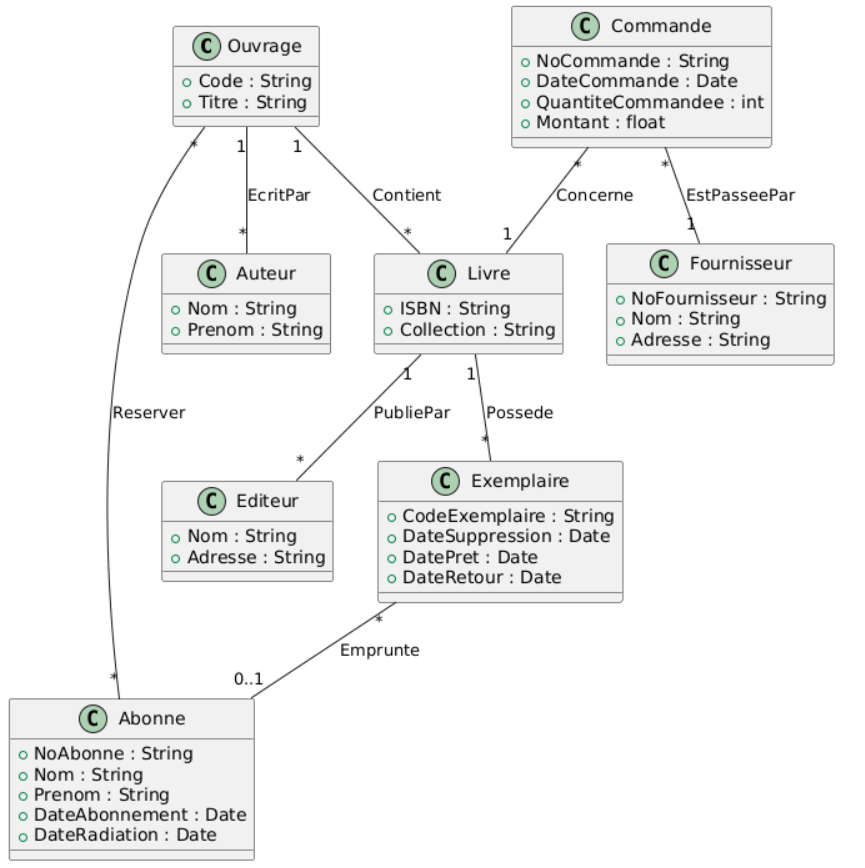
\includegraphics[width=0.8\textwidth]{image.png}
    \caption{Modèle Conceptuel de Données (MCD)}
    \label{fig:mcd}
\end{figure}

\section{Schéma Relationnel}
\begin{itemize}
    \item \textbf{Livre} (\underline{ISBN}, TITRE, NOM EDITEUR, ADRESSE EDITEUR, COLLECTION DU LIVRE)
    \item \textbf{Exemplaire} (\underline{CODE EXEMPLAIRE}, ISBN, DATE DE SUPPRESSION DE L’EXEMPLAIRE)
    \item \textbf{Ouvrage} (\underline{CODE OUVRAGE}, TITRE)
    \item \textbf{Auteur} (\underline{NOM AUTEUR, PRENOM AUTEUR}, CODE OUVRAGE)
    \item \textbf{Abonné} (\underline{N° ABONNE}, NOM ABONNE, PRENOM ABONNE, DATE D'ABONNEMENT, DATE DE RADIATION)
    \item \textbf{Fournisseur} (\underline{N° FOURNISSEUR}, NOM FOURNISSEUR, ADRESSE FOURNISSEUR)
    \item \textbf{Commande} (\underline{N° COMMANDE}, N° FOURNISSEUR, DATE COMMANDE, MONTANT COMMANDE)
    \item \textbf{Commande\_Livre} (\underline{N° COMMANDE, ISBN}, QUANTITÉ COMMANDÉE)
    \item \textbf{Emprunt} (\underline{N° ABONNE, CODE EXEMPLAIRE}, DATE DE PRET DE L’EXEMPLAIRE, DATE DE RETOUR DE L’EXEMPLAIRE)
    \item \textbf{Réservation} (\underline{N° ABONNE, CODE OUVRAGE}, DATE DE RÉSERVATION DE L'OUVRAGE)
\end{itemize}

\end{document}